\documentclass[crop=false,10pt]{standalone}
\usepackage{standard}

\begin{document}
    \begin{figure*}
      \center
      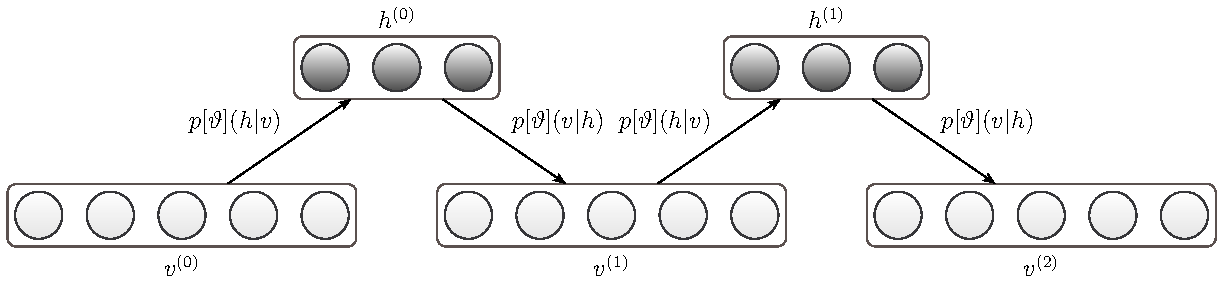
\includegraphics[width=0.9\textwidth]{figures/gibbs-sampling-scheme.pdf}
      \caption{%
        The figure shows the basic scheme of Gibbs sampling.
      }
      \label{fig:gibbs-sampling-scheme}
    \end{figure*}
  \section{Learning} % (fold)
  \label{sec:Learning}

    In this section, we discuss how to estimate the parameters of an RBM, using gradient-based optimizers.
    Generally, RBMs have many parameters and need to be trained on very large datasets.
    Hence, the standard approach taken to learn an RBM is stochastic gradient ascent with the use of mini-batches.
    \cite{Hinton2007,Hinton2010,Murphy2012}

    \subsection{Objective Function} % (fold)
    \label{sub:objective_function}
      Learning is always about optimizing some objective function.
      In a typical FFNN for example one can use cross-entropy as a loss function which then has to be minimized to learn the parameters of the network.
      But in our current mathematical setting we want to learn a probability distribution over the visible values of an RBM.
      For this we have to estimate the parameters based on some given samples.
      In statistics the standard method for estimating the parameters of a statistical model is called maximum likelihood estimation (MLE).
      \cite{Murphy2012}

      Let $n\in\setNatural$ be the number of visible and $m\in\setNatural$ be the number of hidden units for all RBMs in our statistical model.
      Further, let $s\in\setNatural$ be the sample count and define $\mathscr{S} \in \mathscr{B}^{n\times s}$ to be the vector of all samples which are distributed identically and independently.
      Then MLE tries to maximize the probability of the given samples.
      Because of their independence this results in maximizing the product of their probabilities.
      To simplify the analysis further one then typically takes the logarithm of this expression and constructs the log-likelihood function such that every product will be replaced by a sum.
      \[
        \function{\mathscr{L}[\mathscr{S}]}{\setReal^{n\times m + n + m}}{\setReal}
      \]
      \[
        \mathscr{L}[\mathscr{S}](ϑ) \define \frac{1}{s} \sum_{k=1}^s \ln p[ϑ]\roundBrackets{\mathscr{S}_k}
      \]
      Due to the monotonic behavior of the logarithm maximizing the log-likelihood function is equivalent to maximizing the maximum-likelihood function.
      \cite{Murphy2012}
    % subsection objective_function (end)

    \subsection{Gradient Computation} % (fold)
    \label{sub:gradient_computation}
      Because we want to use gradient-based optimizers we now have to compute the derivative of the log-likelihood function with respect to the weight matrix and bias vectors of the RBMs in our statistical model.
      For the sake of simplicity we will only mention the derivative with respect to the weight matrix.
      \[
        \nabla_W \mathscr{L}[\mathscr{S}](ϑ) = \frac{1}{s} \sum_{k=1}^s \expect_ϑ\boxBrackets{\mathscr{V}\transpose{\mathscr{H}} \middle\vert \mathscr{S}_k} - \expect_ϑ\boxBrackets{\mathscr{V}\transpose{\mathscr{H}}}
      \]
      At first sight this formula seems to be complicated.
      But the left part can be easily computed due to the good properties of the posterior probability.
      The right part is much more difficult.
      The typical method of finding such an expectation value of the model itself involves Gibbs sampling.
      Figure \ref{fig:gibbs-sampling-scheme} demonstrates this method schematically.
      \cite{Murphy2012}

      Deriving and explaining the complete procedure of Gibbs sampling would go beyond the scope of this report.
      But Gibbs sampling is generally used to sample from a probability distribution.
      Because an RBM represents such a distribution and we want to estimate a specific expectation value of the model it seems to be the natural choice.
      By using the posterior probability together with visible values we can sample hidden values due to the good properties of an RBM.
      After obtaining some sampled hidden values we do the same thing to generate new visible values.
      In figure \ref{fig:gibbs-sampling-scheme} it becomes clear that we have to repeat this process.
      The main problem lies in the fact that this process takes a long time until it reaches equilibrium and therefore aborting the process too early will result in a bad estimation of the expectation value.
      On the other hand we cannot afford such a computational overhead in the learning process.
      \cite{Murphy2012}
    % subsection gradient_computation (end)

    \subsection{Contrastive Divergence} % (fold)
    \label{sub:contrastive_divergence}
      The idea is now to make rough approximations to the expectation value and to speed up the computation.
      This faster method is known as contrastive divergence (CD).
      To make things good again this algorithm aborts the series after some given number $k\in\setNatural$ and then approximates the expectation value by the following expression.
      Therefore the algorithm is sometimes called $\text{CD}_k$.
      \cite{Hinton2010,Murphy2012}
      \[
        \expect_ϑ\boxBrackets{\mathscr{V}\transpose{\mathscr{H}}} \approx v^{(k)}\transpose{h^{(k)}}
      \]

      Looking at this approximation the learning procedure seems to be unstable and may even diverge in some cases.
      But it is a matter of fact that in reality this algorithm is working efficiently.
      This may be due to the stochastic gradient ascent algorithm which introduces noise in the computation.
      Therefore errors done by CD would average out over multiple iterations of the learning process.
      In \cite{Hinton2010} this is implicitly confirmed because the algorithm shows a much higher performance with a small mini-batch size.
      \cite{Hinton2010,Murphy2012}
    % subsection contrastive_divergence (end)

    \subsection{Application to Collaborative Filtering} % (fold)
    \label{sub:application_to_collaborative_filtering}
      \begin{figure}
        \center
        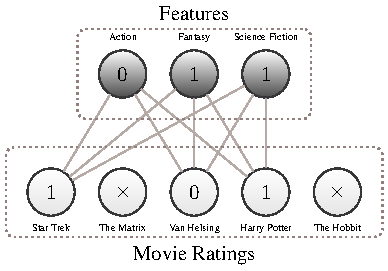
\includegraphics[width=0.441\textwidth]{figures/rbm-learning-example.pdf}
        \caption{%
          The figure shows the application of the learning algorithm to the movie ratings for some user.
        }
        \label{fig:rbm-learning-example}
      \end{figure}
    \begin{figure*}
      \center
      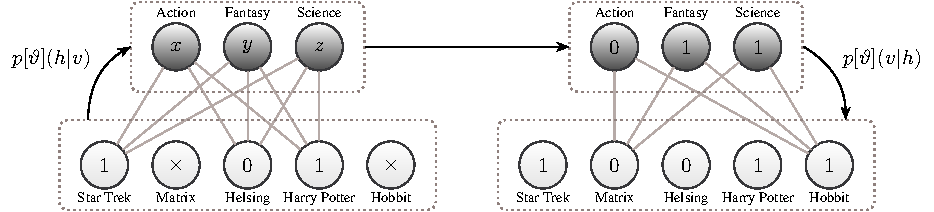
\includegraphics[width=0.9\textwidth]{figures/rbm-inference-example.pdf}
      \caption{%
        The figure shows a schematic example of the application of the inference process to the prediction of movie ratings for a given imaginary user.
        At first, only the rated movies will be used to sample hidden values.
        Then with respect to the sampled hidden values movie ratings for the unrated movies will be sampled and be understood as predictions.
      }
      \label{fig:rbm-inference-example}
    \end{figure*}
      Now one has to talk about the application of the algorithm to collaborative filtering.
      The first problem that arises is that in general every user has rated different movies.
      Hence, we cannot use the same visible units for every user.
      As a solution \cite{Hinton2007} proposed to create an RBM for every user with a constant number of hidden units.
      Then every RBM has one trainings sample, the movie ratings of that user.
      To not have a set of completely independent RBMs we tie the weights and biases of each RBM together such that if two users have rated the same movie then their two RBMs are using the same weights and biases for this visible unit.
      Figure \ref{fig:rbm-learning-example} shows an example for the application of this algorithm for an imaginary user again.
    % subsection application_to_collaborative_filtering (end)
  % section Learning (end)
\end{document}